% vim: set ts=2 sw=2 noet spell:

\chapter{Theory}

\begin{figure}
	\centering
	\resizebox{.9\linewidth}{!}{
		% vim: set ts=2 sw=2 noet spell:

\begin{tikzpicture}[
		% show background rectangle,
		box/.style = {
			font = \small\sffamily\bfseries,
			draw, thick, fill = white,
			minimum height = 10mm,
			minimum width = 25mm,
		},
	]
	\matrix[
		nodes = {box}, column sep = 10mm, row sep = 10mm,
	]{
		\node (SRC) {Source}; &
		\node (ENC) {Encoder}; &
		\node (MOD) {Modulator}; \\
		&& \node (CHN) {Channel}; \\
		\node (SNK) {Sink}; &
		\node (DEC) {Decoder}; &
		\node (DMD) {Demodulator}; \\
	};
	\draw[very thick, -latex]
		(SRC) edge node[midway, above] {\(m\)}    (ENC)
		(ENC) edge node[midway, above] {\(m_e\)}  (MOD)
		(MOD) edge node[midway, right] {\(s\)}    (CHN)
		(CHN) edge node[midway, right] {\(y\)}    (DMD)
		(DMD) edge node[midway, above] {\(m_e'\)} (DEC)
		(DEC) edge node[midway, above] {\(m'\)}   (SNK)
	;

	\draw[very thick, -latex]
		($(MOD.east)+(5mm,0)$) node[right] (CARR) {Carrier \(e^{j(\omega_c t + \phi)}\)} to (MOD);

	\draw[very thick, -latex]
		($(CHN.east)+(5mm,0)$) node[right] (NOISE) {Noise \(n\)} to (CHN);

	% \draw[very thick, -latex]
	% 	($(CHN.west)-(5mm,0)$) node[left] (FADE) {Fading} to (CHN);

	\draw[very thick, -latex]
		($(DMD.east)+(5mm,0)$) node[right] (SYNC) {Sync} to (DMD);

	\begin{pgfonlayer}{background}
		\fill[lightgray!20] ($(SRC.north west)+(-5mm,5mm)$) node (TX) {}
			rectangle ($(MOD.south -| CARR.east)+(5mm,-5mm)$);

		\fill[lightgray!20] ($(SNK.north west)+(-5mm,5mm)$) node (RX) {}
			rectangle ($(DMD.south -| CARR.east)+(5mm,-5mm)$);

		\node[gray, font = \sffamily\bfseries, anchor = south west]
			at (TX.north) {Transmitter};

		\node[gray, font = \sffamily\bfseries, anchor = south west]
			at (RX.north) {Receiver};
	\end{pgfonlayer}
\end{tikzpicture}

	}
	\caption{
		Block diagram of our wireless communication system with annotated signal names. Frequency domain representations of signals use the uppercase symbol of their respective time domain name.
		\label{fig:notation}
	}
\end{figure}

\section{Overview}

The following two sections will briefly introduce mathematical formulations of the modulation schemes and of the channel models used in this project. The notation used is summarised in \figref{fig:notation}. For conciseness encoding schemes and (digital) signal processing calculations are left out and discussed later.  Section \ref{sec:multipath-fading} presents an established mathematical model to understand multipath fading, as well as a brief description of a discrete-time model and the intricacies caused by the sampling process. Finally the concept of stochastic models is mentioned, as they are often used to simulate multipath channels \cite{Messier,Mathis}.

%% TODO: A section on maths?
% \section{Signal space and linear operators}

\section{Quadrature amplitude modulation (\(M\)-ary QAM)}

\begin{figure}
	\centering
	\resizebox{\linewidth}{!}{
		% vim: set ts=2 sw=2 noet:

\begin{circuitikz}[
	]
	\matrix [
		row sep = 5mm, column sep = 7mm,
		nodes = {
			align = center,
			fill = white,
		},
	] {
		& \coordinate (vmi);
			& \node[twoportshape] (B2Li) {};
			&
			& \coordinate (mi);
			&
			& \node[mixer] (Mi) {};
			& \coordinate (si);
			\\
		\node[] (M) {\(m(n)\)};
			& \node[twoportshape] (BSp) {};
			&
			&
			& \node[twoportshape] (H) {};
			& \node[oscillator] (OSC) {};
			& \coordinate (phii);
			& \node[adder] (SUM) {};
			& \node (S) {\(s(t)\)};
			\\
		&&&& \coordinate (phiq);
			\\[-3mm]
		& \coordinate (vmq);
			& \node[twoportshape] (B2Lq) {};
			& \coordinate (mq);
			& \node[mixer] (Mq) {};
			&
			&
			& \coordinate (sq);
			\\
	};

	% Add missing lables
	\node at (H.center) {\large \(\mathcal{H}\)};
	\node at (B2Li.center) {\textsf{B2L}};
	\node at (B2Lq.center) {\textsf{B2L}};
	\node at (BSp) {\textsf{BSp}};

	% Add connections
	\begin{scope}[thick, -latex]
		\draw (M) -- (BSp.west);

		\draw (BSp.north) |- (B2Li.west);
		\draw (B2Li.east) -- (Mi.west);
		\draw (Mi.east) -| (SUM.north);

		\draw (BSp.south) |- (B2Lq.west);
		\draw (B2Lq.east) -- (Mq.west);
		\draw (Mq.east) -| (SUM.south);

		\draw (SUM) -- (S);

		\draw (OSC.east) -| (Mi.south);
		\draw (OSC.west) -- (H.east);
		\draw (H.south) -- (Mq.north);
	\end{scope}

	% Add signal labels
	\node[above right] at (vmi) {\(\vec{m}_i\)};
	\node[below right] at (vmq) {\(\vec{m}_q\)};

	\node[above] at (mi) {\(m_i(t)\)};
	\node[below] at (mq) {\(m_q(t)\)};

	\node[above right] at (phii) {\(\phi_i\)};
	\node[right, yshift = 1mm] at (phiq) {\(\phi_q\)};

	\node[above left] at (si) {\(s_i(t)\)};
	\node[below left] at (sq) {\(s_q(t)\)};

	\begin{pgfonlayer}{background}
		\fill[left color = white, right color = blue!20, draw = white]
			($(B2Li.north) + (0,1)$) coordinate (D) rectangle ($(B2Lq.south) - (3,1)$);
		\fill[right color = white, left color = red!20, draw = white]
			($(B2Li.north) + (0,1)$) coordinate (A) rectangle ($(B2Lq.south) + (9,-1)$);

		\node[blue!50, anchor = south east, xshift = -4mm] at (D) {\bfseries\ttfamily Digital bits};
		\node[red!50, anchor = south west, xshift = 4mm]  at (A) {\bfseries\ttfamily Analog waveform};
	\end{pgfonlayer}
\end{circuitikz}

	}
	\caption{
		Block diagram of a \(M\)-ary QAM modulator.
		\label{fig:quadrature-modulation}
	}
\end{figure}

Quadrature amplitude modulation is a family of modern digital modulation methods, that use an analog carrier signal. The simple yet effective idea behind QAM is to encode extra information into an orthogonal carrier signal, thus increasing the number of bits sent per unit of time (symbol) \cite{Gallager,Kneubuehler,Mathis,Hsu}. A block diagram of the process is shown in \figref{fig:quadrature-modulation}.

%% TODO: Quick par on "we will dicusss M-Ary QAM, M is 2^something"

\subsection{Modulation of a digital message}

\paragraph{Bit splitter}

As mentioned earlier, quadrature modulation allows sending more than one bit per unit time. The first step is to use a so called bit splitter, that converts the continuous bitstream \(m(n)\) into pairs of chunks of \(\sqrt{M}\) bits each. The two bit vectors of length \(\sqrt{M}\), denoted by \(\vec{m}_i\) and \(\vec{m}_q\) in figure \ref{fig:quadrature-modulation}, are called in-phase and quadrature component respectively\cite{Hsu}. The reason will become more clear later.

\paragraph{Binary to level converter}

%% TODO: explain why gray code

Both bit vectors \(\vec{m}_i, \vec{m}_q \in \{0,1\}^{\sqrt{M}}\) are sent through a binary to level converter. It's purpose is to reinterpret the bit vectors as numbers, usually in gray code, and to convert them into analog waveforms, which we will denote with \(m_i(t)\) and \(m_q(t)\) respectively. Mathematically the binary to level converter can be described as:
\begin{equation}
	m_i(t) = \text{Level}(\vec{m}_i) \cdot p(t),
\end{equation}
i.e. a pulse function\footnote{Typically a root raised cosine to optimize for bandwidth \cite{Hsu}.} \(p(t)\) scaled by the interpreted binary value, written here using a ``Level'' function. So at this point a level of each analog waveform is encodes \(\sqrt{M}\) bits per unit time, and there are two of such waveforms.


\paragraph{Mixer}

Having analog level signals, it is this now possible to mix them with radio frequency carriers. Because there are two waveforms, one might expect that two carrier frequencies are necessary, however this is not the case. The two component \(m_i(t)\) and \(m_q(t)\) are mixed with two different periodic signals \(\phi_i(t)\) and \(\phi_q(t)\) that have the same frequency \(\omega_c = 2\pi / T\). How this is possible is explained in the next section.


\subsection{Orthogonality of carrier signals}

Before explaining how the two carrier signals are generated, we first need to discuss some important mathematical properties \(\phi_i\) and \(\phi_q\) need to have, in order to modulate two messages over the same frequency \(\omega_c\). The two carriers need to be \emph{orthonormal}\footnote{Actually orthogonality alone would be sufficient, however then the left side of \eqref{eqn:orthonormal-condition} would not equal 1, and an inconvenient factor would be introduced in many later equations \cite{Gallager,Hsu}.} to each other, mathematically this is expressed by the conditions
\begin{subequations} \label{eqn:orthonormal-conditions}
	\begin{align}
		\langle \phi_i, \phi_q \rangle
			&= \int_T \phi_i \phi_q^* \, dt
			= 0, \text{ and } \label{eqn:orthogonal-condition} \\
		\langle \phi_k, \phi_k \rangle
			&= \int_T \phi_k \phi_k^*  \,dt = 1,
			\text{ where } k \text{ is either } i \text{ or } q. \label{eqn:orthonormal-condition}
	\end{align}
\end{subequations}
Provided these rather abstract conditions, let's define a new signal 
\begin{equation}
	s = m_i\phi_i + m_q\phi_q.
\end{equation}
%% TODO: is this assumption correct?
Notice that assuming \(m_i\) and \(m_q\) are constant\footnote{This is an approximation assuming that the signal changes much slower relative to the carrier.} over the carrier's period \(T\),
\begin{align*}
	\langle s, \phi_i \rangle = \int_T s \phi_i^* \,dt
		&= \int m_i \phi_i \phi_i^* + m_q \phi_q \phi_i^* \,dt \\
		&= m_i \underbrace{\int_T \phi_i \phi_i^* \,dt}_{1}
			+ m_q \underbrace{\int_T \phi_q \phi_i^* \,dt}_{0} = m_i,
\end{align*}
which effectively means that it is possible to isolate a single component \(m_i(t)\) out of \(s(t)\). The same of course works with \(\phi_q\) as well resulting in \(\langle s, \phi_q \rangle = m_q\). Thus (remarkably) it is possible to send two signals on the same frequency, without them interfering with each other. Since each signal can represent one of \(\sqrt{M}\) values, by having two we obtain \(\sqrt{M} \cdot \sqrt{M} = M\) possible combinations.

A graphical way to see what is happening, is to observe a so called \emph{constellation diagram}. An example is shown in \figref{fig:qam-constellation} for \(M = 16\). The two carrier signals \(\phi_i\) and \(\phi_q\) can be understood as bases of a coordinate system, in which the two amplitude levels of the two modulated messages, determine a position in the grid.

\paragraph{Example}

A concrete example for \(M = 16\): if the message is 1110 the bit splitter creates two values \(\vec{m}_q = 11\) and \(\vec{m}_i = 10\); both are converted into analog amplitudes (symbols) \(m_q = 3\) and \(m_i = 4\); that are then mixed with their respective carrier, resulting in \(s(t)\) being the point inside the bottom right sub-quadrant of the top right quadrant (blue dot in \figref{fig:qam-constellation}).

In \figref{fig:qam-constellation} the dots of the constellation have coordinates that begin on the bottom left corner, and are nicely aligned on a grid. Both are not a necessary requirement for QAM, in fact there are many schemes (for example when \(M = 32\)) that are arranged on a non square shape, and place the dots in different orders. The only constraint that most QAM modulators have in common, with regards to the geometry of the constellation, is that between any two adjacent dots (along the axis, not diagonally) only one bit of the represented value changes (gray code). This is done to improve the bit error rate (BER) of the transmission.

\begin{figure}
	\hfill
	\begin{subfigure}{.4\linewidth}
		% vim: set ts=2 sw=2 noet:
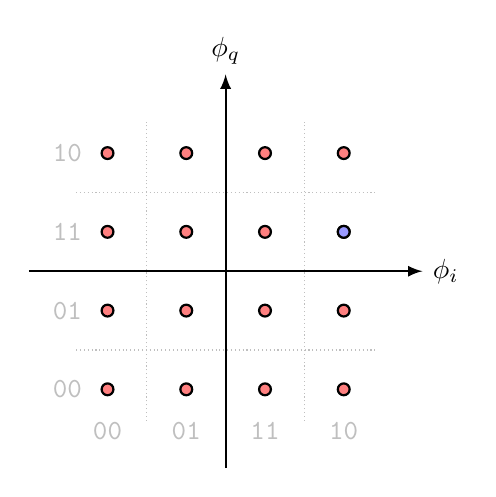
\begin{tikzpicture}[
		axis/.style = {
			thick, -latex, black,
		},
		star/.style = {
			draw = black, thick, fill = red!50,
			circle, outer sep = 1mm, inner sep = 0,
			minimum size = 1.5mm,
		},
	]

	\draw[lightgray, densely dotted, step = 10mm] (-19mm,-19mm) grid (19mm,19mm);

	\draw[axis] (-25mm,0) to (25mm,0) node[right] {\(\phi_i\)};
	\draw[axis] (0,-25mm) to (0,25mm) node[above] {\(\phi_q\)};

	\foreach \i in {0,1,...,3}{
		\foreach \q in {0,1,...,3}{
			\node[star] (s\i\q) at ({\i*10mm - 15mm},{\q*10mm - 15mm}) {};
		}
	}

	% special node for the example
	\node[star, fill = blue!40!white] at (s32) {};

	\foreach \i/\l in {0/00,1/01,2/11,3/10}{
		\node[lightgray, below = 3mm] at (s\i0) {\texttt{\l}};
		\node[lightgray, left = 2mm] at (s0\i) {\texttt{\l}};
	}
\end{tikzpicture}

		\caption{16-QAM\label{fig:qam-constellation}}
	\end{subfigure}
	\hfill
	\begin{subfigure}{.4\linewidth}
		% vim: set ts=2 sw=2 noet:
\begin{tikzpicture}[
		axis/.style = {
			thick, -latex, black,
		},
		star/.style = {
			draw = black, thick, fill = red!50,
			circle, outer sep = 1mm, inner sep = 0,
			minimum size = 1.5mm,
		},
	]
	\draw[axis] (-25mm,0) to (25mm,0) node[right] {\(\phi_i\)};
	\draw[axis] (0,-25mm) to (0,25mm) node[above] {\(\phi_q\)};

	\draw[lightgray, densely dotted, thick] (0,0) circle (15mm);
	\foreach \a in {0,1,...,8}{
		\node[star] (s\a) at ({360/8*(.5 + \a)}:15mm) {};
	}

	\foreach \i/\l in {0/000,1/001,2/011,3/010,4/110,5/111,6/101,7/100}{
		\node[lightgray] at ($(s\i) + ({360/8*(.5 + \i)}:5mm)$) {\texttt{\l}};
	}
\end{tikzpicture}

		\caption{8-PSK\label{fig:psk-constellation}}
	\end{subfigure}
	\hfill
	\caption{
		Examples of constellation diagrams. Each dot represents a possible location for the complex amplitude of the passband signal.
	}
\end{figure}

\subsection{Construction of orthogonal carrier signals}

Knowing why there is a need for orthogonal carriers, we should now discuss which functions satisfy the property described by \eqref{eqn:orthogonal-condition}. If \(\phi_i\) is a real valued signal (which is typical) it is possible to find a function the quadrature carrier using the \emph{Hilbert transform} (sometimes called Hilbert filter):
\begin{equation}
	\hilbert g(t) = g(t) * \frac{1}{\pi t}
		= \frac{1}{\pi} \int_\mathbb{R} \frac{g(\tau)}{t - \tau} \,d\tau
		= \frac{1}{\pi} \int_\mathbb{R} \frac{g(t - \tau)}{\tau} \,d\tau.
\end{equation}
The Hilbert transform is a linear operator that introduces a phase shift of \(\pi / 2\) over all frequencies \cite{Hsu,Gallager}, and it is possible to show that given a real valued function \(g(t)\) then \(\langle g, \hilbert g \rangle = 0\) \cite{Kschischang,Kneubuehler}. There are many functions that are Hilbert transform pairs, however in practice the pair \(\phi_i(t) = \cos(\omega_c t)\) and \(\phi_q(t) = \hilbert \phi_i(t) = \sin(\omega_c t)\) is always used.

% \paragraph{Oscillator and phase shifter}
% \skelpar[4]{Give a few details on how the carrier is generated in practice.}

% \subsection{Spectral properties of a QAM signal}
% \skelpar[4]{Spectral properties of QAM}

\section{Phase shift keying (\(M\)-PSK)}

Phase shift keying (PSK) is another popular family of modulation schemes for digital signals, that is however simpler than QAM. In PSK as the name suggests only the phase of the envelope changes, which means that the symbols have all the same amplitude. Thus, instead of arranging the symbols into a grid as done in QAM, \(M\)-PSK distributes the symbols over the unit circle at equidistant intervals of \(2\pi / M\) radians \cite{Mathis,Kneubuehler}. An example of 8-PSK is shown in \figref{fig:psk-constellation}. Mathematically the process of a PSK modulation can be described by \skelpar[2]
\begin{equation}
	\skelpar[1]
\end{equation}
\skelpar[3]

% \begin{figure}
% 	% TODO: Better Image
% 	% https://sites.google.com/site/billmahroukelec675/bipolar-phase-shift-keying
% 	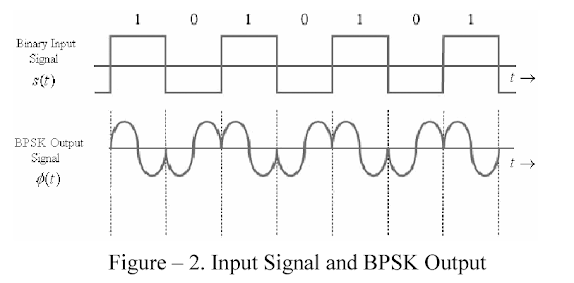
\includegraphics[width=5cm]{./image/BPSK2.png}
% \end{figure}

\subsection{Quadrature PSK (QPSK)}

\skelpar[2]{QPSK = 4-PSK = 4-QAM}

\section{Multipath fading} \label{sec:multipath-fading}

In the previous section, we discussed how the data is modulated and demodulated at the two ends of the transmission system. This section discusses what happens between the sender and receiver when the modulated passband signal is transmitted wirelessly.

In theory because wireless transmission happens through electromagnetic radiation, to model a wireless channel one would need to solve Maxwell's equations for either the electric or magnetic field, however in practice that is not (analytically) possible. Instead what is typically done, is to model the impulse response of the channel using a geometrical or statistical model, parametrized by a set of coefficients that are either simulated or measured experimentally \cite{Gallager}.

In our relatively simple model we are going to include an additive white Gaussian noise (AWGN) and a Rician (or Rayleighan) fading; both are required to model physical effects of the real world. The former in particular is relevant today, as it mathematically describes dense urban environments.

\subsection{Geometric model}

The simplest way to understand the multipath fading, is to consider it from a geometrical perspective. \figref{fig:multipath-sketch} is a sketch a wireless transmission system affected by multipath fading. The sender's antenna radiates an electromagnetic wave in the direction of the receiver (red line), however even under the best circumstances a part of the signal is dispersed in other directions (blue lines).

\begin{figure}
	\centering
	% vim: set ts=2 sw=2 noet:
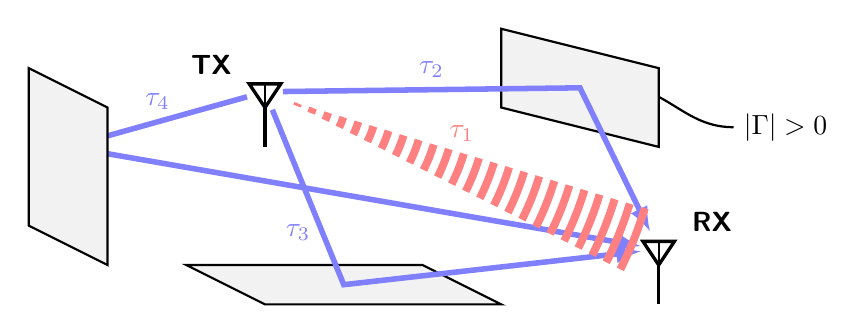
\begin{tikzpicture}[
			antenna/.pic = {
				\draw[very thick] (0,0) -- ++(2mm, 3mm) -- ++(-4mm,0) -- cycle;
				\draw[very thick] (0,0) -- ++(0,-5mm) coordinate (-mast) {};
				\draw[thick] (0,0) -- ++(0,3mm);
				\node[inner sep = 0pt, outer sep = 6pt] (-center) at (0,2mm) {};
			},
	]

	% Antennas
	\draw (0,2) pic (T) {antenna} node[above left = 3mm] {\sffamily\bfseries TX};
	\draw (5,0) pic (R) {antenna} node[above right = 3mm] {\sffamily\bfseries RX};

	% wall coefficients
	\draw[thick] (4.75, 2.25) to[out = -20, in = 180] ++(1.2,-.5) node[right] {\(|\Gamma| > 0\)};

	% walls
	\draw[thick, fill = lightgray!20] (3,2) -- ++(2,-.5) -- ++(0,1) -- ++(-2,.5) -- cycle;
	\draw[thick, fill = lightgray!20] (-1,0) -- ++(3,0) -- ++(1,-.5) -- ++(-3,0) -- cycle;


	% reflected signals
	\draw[line width = 2pt, blue!50!white, -latex] (T-center) -- node[above, pos = .5] {\(\tau_2\)} (4,2.25) -- (R-center);
	\draw[line width = 2pt, blue!50!white, -latex] (T-center) -- node[left, pos = .7] {\(\tau_3\)} (1,-.25) -- (R-center);
	\draw[line width = 2pt, blue!50!white, -latex] (T-center) -- node[above, pos = .5] {\(\tau_4\)} (-2.5,1.5) -- (R-center); 

	% another wall
	\draw[thick, fill = lightgray!20] (-2,0) -- ++(-1,.5) -- ++(0,2) --++(1,-.5) -- cycle;

	% LOS path
	\draw[line width = 1mm, red!50!white,
		decorate, decoration = {
			expanding waves, angle = 5, segment length = 2mm
		}
	] (T-center) -- node[above = 2mm, pos = .5] {\(\tau_1\)} (R-center);
\end{tikzpicture}

	\caption{
		Sketch of channel with multipath fading.
		\label{fig:multipath-sketch}
	}
\end{figure}

The problem is that, as is geometrically evident, some paths are longer than others. Because of this fact, the signal is seen by the receiver multiple times with different phase shifts \cite{Gallager,Messier}. To mathematically model this effect, we describe the received signal \(r(t)\) as a linear combination of delayed copies of the sent signal \(s(t)\), each with a different attenuation \(c_k\) and phase shift \(\tau_k\):
\begin{equation} \label{eqn:geom-multipath-rx}
	r(t) = \sum_k c_k s(t - \tau_k).
\end{equation}

The linearity of the model is justified by the assumption that the underlying electromagnetic waves behave linearly (superposition holds) \cite{Gallager}. How many copies of \(s(t)\) (usually referred to as ``taps'' or ``rays'') should be included in \eqref{eqn:geom-multipath-rx}, depends on the precision requirements of the model.

A further complication arises, when one end (or both) is not stationary. In that case the lengths of the paths change over time, and as a result both the delays \(\tau_k\) as well as the attenuations \(c_k\) become functions of time: \(\tau_k(t)\) and \(c_k(t)\) respectively \cite{Gallager,Messier}. Even worse when the velocity at which the device is moving is high, then Doppler shifts of the electromagnetic wave frequency become non negligible \cite{Gallager}.

\begin{figure}
	\centering
	% vim: set ts=2 sw=2 noet:
\tdplotsetmaincoords{70}{40}
\begin{tikzpicture}[tdplot_main_coords, font = \footnotesize\ttfamily]
	\draw[thick, -latex] (0,0,0) -- node[sloped, midway, below, gray] {Effect of the channel} (7,0,0) node[right] {\(\tau\)};
	\draw[thick, -latex] (0,0,0) -- node[sloped, midway, above, gray] {How the channel changes} (0,7,0) node[right] {\(t\)};
	\draw[thick, -latex] (0,0,0) -- (0,0,2) node[above] {\(h(t,\tau)\)};

	\foreach \y in {1,2,...,4}{
		\draw[dashed, gray] (0,1.5*\y,0) -- ++(7,0,0);
	}

	\foreach \x in {1,2,...,6}{
		\draw[dotted, gray] (\x,0,0) -- ++(0,7,0);
	}

	% draw 4 responses
	\begin{scope}[very thick, -{Circle[fill=white]}]
		\foreach \x/\v in {.8/1, 2.2/2, 2.9/1, 4/4, 5.1/7, 5.8/3}{
			\draw[blue!80!red] (\x,1.5*4,0) -- ++(0,0,\v/3);
		}

		\foreach \x/\v in {.9/2, 2.1/2, 3/1, 4/3, 5/6, 6/3}{
			\draw[blue!60!red] (\x,1.5*3,0) -- ++(0,0,\v/3);
		}

		\foreach \x/\v in {.6/1, 2/1, 2.8/3, 4.1/4, 5.5/4, 6.2/1}{
			\draw[blue!40!red] (\x,1.5*2,0) -- ++(0,0,\v/3);
		}

		\foreach \x/\v in {1.1/2, 1.8/1, 3/2, 3.7/1, 4.8/3, 5.8/1}{
			\draw[blue!20!red] (\x,1.5,0) -- ++(0,0,\v/3);
		}
	\end{scope}
\end{tikzpicture}

	\caption{
		LTV impulse response of a multipath fading channel.
		\label{fig:multipath-impulse-response}
	}
\end{figure}

We have thus observed that the arrangement can be modelled as a linear time-\emph{varying} system (LTV), if the sender or the receiver (or anything else in the channel) is moving, and as a linear time \emph{invariant} (LTI) system if the geometry is stationary. Regardless of which of the two cases, linearity alone is sufficient to approximate the channel as finite impulse response (FIR) filter \cite{Messier}. We can rewrite LTV version of equation \eqref{eqn:geom-multipath-rx} using a convolution product as following:
\begin{align*}
	r(t) = \sum_k c_k(t) s(t - \tau_k(t)) &= \sum_k c_k(t) \int_\mathbb{R} s(\tau) \delta(\tau - \tau_k(t)) \,d\tau \\
		&= \int_\mathbb{R} s(\tau) \sum_k c_k(t) \delta(\tau - \tau_k(t)) \,d\tau = s(\tau) * h(\tau, t),
\end{align*}
obtaining a new function
\begin{equation} \label{eqn:multipath-impulse-response}
	h(\tau, t) = \sum_k c_k(t) \delta(\tau - \tau_k(t)),
\end{equation}
that describes the \emph{channel impulse response} (CIR). This function depends on two time parameters: actual time \(t\) and convolution time \(\tau\). To better understand \(h(\tau, t)\), consider an example shown in figure \ref{fig:multipath-impulse-response}. Each stem represents a weighted Dirac delta, so each series of stems of the same color, along the convolution time \(\tau\) axis, is a channel response at some specific time \(t\). Along the other axis we see how the entire channel response changes over time\footnote{In the figure only a finite number of stems was drawn, but actually the weights \(c_k(t)\) of the Dirac deltas change continuously.}. Notice that the stems are not quite aligned to the \(\tau\) time raster (dotted lines), that is because in \eqref{eqn:multipath-impulse-response} not only the weights \(c_k\) but also the delays \(\tau_k\) are time dependent.

\subsection{Spectrum of a multipath fading channel}

With a continuous time channel model we can now discuss the spectral properties of a fading channel since the frequency response is the Fourier transform of the impulse response, mathematically \(H(f, t) = \fourier h(\tau, t)\). In this case however \(h(\tau, t)\) depends on two time variables, but that is actually not an issue, it just means that the frequency response is also changing over time. Hence we perform the Fourier transform with respect to the channel (convolution) time variable \(\tau\) to obtain
\begin{equation} \label{eqn:multipath-frequency-response}
	H(f, t) = \int_\mathbb{R} \sum_k c_k(t) \delta(\tau - \tau_k(t)) e^{-2\pi jf\tau} \, d\tau
	= \sum_k c_k(t) e^{-2\pi jf \tau_k(t)}.
\end{equation}

Equation \eqref{eqn:multipath-frequency-response} shows that the frequency response is a periodic complex exponential, which has some important implications. Notice that if there is only one tap (term), the magnitude of \(H(f, t)\) is a constant (with respect to \(f\)) since \(|e^{j\alpha f}| = 1\). This means that the channels attenuates all frequencies by the same amount, therefore it is said to be a \emph{frequency non-selective} or \emph{flat fading} channel. Whereas in the case when there is more than one tap, the taps interfere destructively at certain frequencies and the channel is called \emph{frequency selective}. To illustrate how this happens, plots of the frequency response of a two tap channel model are shown in \figref{fig:multipath-frequency-response-plots}. On the left is the magnitude of \(H(f, t)\), which presents periodic ``dips'', and on the right complex loci for the two taps (red and blue), as well as their sum (magenta), over the frequency range near the first dip (2 to 2.5 MHz) are shown.


\begin{figure}
	\centering
	\resizebox{\linewidth}{!}{
		% vim: set ts=2 sw=2 noet:
\begin{tikzpicture}
	\begin{loglogaxis}[
			width = .6\linewidth, height = 5cm,
			ylabel = {Response \(|H(f, t)|\)},
			xlabel = {Frequency \(f\)/Hz},
			xlabel near ticks,
			ylabel near ticks,
			ytick = \empty,
			smooth,
		]

		\addplot[solid, magenta] table[x index = 0, y index = 2]
			{figures/data/multipath_frequency_response.dat};
		% \addlegendentry{Multipath}

		% \addplot[dashed, thick, black] table[x index = 0, y index = 1]
		% 	{figures/data/multipath_frequency_response.dat};
		% \addlegendentry{Linear}

	\end{loglogaxis}
\end{tikzpicture}
\hskip 5mm
\begin{tikzpicture}[
		decorated/.style = {
			solid, thick,
			postaction={decorate},
			decoration={markings,
				mark=at position 0.35 with {\arrow{stealth}},
				mark=at position 0.65 with {\arrow{stealth}}},
		},
	]
	\begin{axis}[
			width = 5cm, height = 5cm,
			ylabel = {\(\Im{H(f,t)}\)},
			xlabel = {\(\Re{H(f,t)}\)},
			xlabel near ticks,
			ylabel near ticks,
			grid = major,
			xmin = -1.2, xmax = 1.2,
			ymin = -1.2, ymax = 1.2,
		]

		\addplot[decorated, red] table[x index = 3, y index = 4]
			{figures/data/multipath_frequency_response.dat}
			node[pos = 0, circle, fill = white, draw, inner sep = 1pt] {}
			node[pos = .2, outer sep = 1pt, inner sep = 0pt] (A) {}
			node[pos = 1, circle, fill = white, draw, inner sep = 1pt] {};

		\addplot[decorated, blue] table[x index = 5, y index = 6]
			{figures/data/multipath_frequency_response.dat}
			node[pos = 0, circle, fill = white, draw, inner sep = 1pt] {}
			node[pos = .2, outer sep = 1pt, inner sep = 0pt] (B) {}
			node[pos = 1, circle, fill = white, draw, inner sep = 1pt] {};

		\addplot[decorated, magenta] table[x index = 7, y index = 8]
			{figures/data/multipath_frequency_response.dat}
			node[pos = 0, circle, fill = white, draw, inner sep = 1pt] {}
			node[pos = 0, below right, font = \tiny] {2 MHz}
			node[pos = .2, outer sep = 1pt, inner sep = 0pt] (C) {}
			node[pos = 1, circle, fill = white, draw, inner sep = 1pt] {}
			node[pos = 1, above left, font = \tiny] {2.5 MHz};

		\node[outer sep = 2pt, inner sep = 0pt] (O) at (0,0) {};
		\draw[-latex, red!50!white] (O) -- (A);
		\draw[-latex, blue!50!white] (O) -- (B);
		\draw[-latex, magenta!50!white] (O) -- (C);

	\end{axis}
\end{tikzpicture}

		% \skelfig[width = .8 \linewidth, height = 3cm]{}
	}
	\caption{
		Frequency response of a multipath fading channel.
		\label{fig:multipath-frequency-response-plots}
	}
\end{figure}

\subsection{Quantifying dispersion}

Having discussed how multipath fading affects communication systems, the next important step is to be able quantify its effects to be able to compare different multipath channels to each other.

An intuitive parameter to quantify how dispersive channel is, is to take the time difference between the fastest and slowest paths with significant energy. What in the literature is called \emph{delay spread}, and is denoted here by \(T_d\). Consequently, a low delay spread means that all paths have more or less the same length, while a high delay spread implies that there is a large difference in length among the paths. Thus \(T_d\) could be be defined as
\begin{equation}
	T_d = \max_{k} (\tau_k(t)) -  \min_{k} (\tau_k(t)),
\end{equation}
as is done in \cite{Gallager}. However since in reality some paths get more attenuated than others (\(c_k(t)\) parameters) it also not uncommon to define the delay spread as a weighted mean or even as a statistical second moment (RMS value), where mean tap power \(\expectation\{|c_k(t)|^2\}\) is taken into account \cite{Mathis,Messier}. % More sophisticated definitions of delay spread will be briefly mentioned later in section \ref{sec:statistical-model}.

Another important parameter for quantifying dispersion is \emph{coherence bandwidth}, a measure that is highly related to delay spread but in the frequency domain. % Coherence bandwidth can be be defined as 
\skelpar[3]

% \subsection{Effects of multipath fading on modulation constellations}
% 
% % TODO : Can we sai it that way /dose it need to be in the implementation Part?
% 
% It is to mention that not every constellation of parameter for a fading illustration leads to a satisfying  plot constellation.
% For example in a Discrete-time Model: the same delay as the samples per Symbol or a multiple of it leads to a special case, where we see the constellation are around the modulate signal points, when there is no line of side path. This is because of \skelpar{Beschreiben warnn die Werte hübsch sind}

\subsection{Discrete-time model} \label{sec:discrete-time-model}

% TODO: discuss the "bins" of discrete time

Since in practice signal processing is done digitally, it is meaningful to discuss the properties of a discrete-time model. To keep the complexity of the model manageable some assumptions are necessary, thus the sent discrete signal\footnote{This is an abuse of notation. The argument \(n\) is used to mean the \(n\)-th digital sample of \(s\), whereas \(s(t)\) is used for the analog waveform. A more correct but longer notation is \(s(nT)\), where \(T\) is the sample time.} \(s(n)\) is assumed to have a finite single sided bandwidth \(W\). This implies that in the time-domain signal is a series of sinc-shaped pulses each shifted from the previous by a time interval \(T = 1 / (2W)\) (Nyquist rate):
\begin{equation}
	s(t) = \sum_n s(n) \sinc(t/T - n)
\end{equation}
The waveform \(s(t)\) is then convolved with the CIR function \(h(\tau, t)\) (with respect to \(\tau\)) from the continuous time model resulting in the waveform at the receiver
\begin{align*}
	r(t) &= \int_ \mathbb{R} \sum_n s(n) \sinc(\tau / T - n) \sum_k c_k(t) \delta(\tau - \tau_k(t)) \,d\tau \\
	&= \sum_n s(n) \sum_k c_k(t) \sinc(t/T - \tau_k(t)/T - n),
\end{align*}
which is then sampled at the Nyquist rate of \(2W = 1/T\), resulting in a set of samples\footnote{Again, the abusing notation \(r(m)\) means the \(m\)-th digital sample of \(r(t)\), i.e. \(r(mT)\).}:
\[
	r(m) = \sum_n s(n) \sum_k c_k(mT) \sinc(m - \tau_k(mT)/T - n).
\]
Finally the substitution \(l = m - n\) eliminates the sender's sample counter \(n\) (unknown to the receiver) and reformulates \(r(m)\) as a discrete convolution product of with a discrete CIR function \(h_l(m)\):
\begin{equation}
	r(m) = \sum_l s(m - l) \sum_k c_k(mT) \sinc(l - \tau_k(mT)/T) 
	= \sum_l s(m - l) h_l (m).
\end{equation}
This result is very similar to the continuous time model described by \eqref{eqn:multipath-impulse-response} in the sense that each received digital sample is a sent sample convolved with a different discrete channel response (because of time variance). To see how the discrete CIR
\begin{equation} \label{eqn:discrete-multipath-impulse-response}
	h_l(m) = \sum_k c_k(mT) \sinc(l - \tau(mT)/T)
\end{equation}
is different from \eqref{eqn:multipath-impulse-response} consider again the plot of \(h(\tau,t)\) in \figref{fig:multipath-impulse-response}. The plot of \(h_l(m)\) would have discrete axes with \(m\) replacing \(t\) and \(l\) instead of \(\tau\), and because of the finite bandwidth in the \(l\) axis instead of Dirac deltas there would be superposed sinc functions.

\begin{figure}
	\centering
	% vim: set ts=2 sw=2 noet:
\begin{tikzpicture}[
		dot/.style = {
			circle,
			fill = black, draw = black,
			minimum size = 1.5mm,
			outer sep = 0, inner sep = 0,
		},
		block/.style = {
			rectangle, draw, thick,
			black, fill = white,
			minimum height = 8mm, minimum width = 8mm,
		},
		prod/.style = {
			circle, draw, thick,
			black, fill = white,
			minimum size = 6mm,
			inner sep = 0, outer sep = 0,
		},
		sum/.style = {
			circle, draw, thick,
			black, fill = white,
			minimum size = 6mm,
			inner sep = 0, outer sep = 0,
		},
	]

	\matrix[column sep = 5mm, row sep = 3mm] {
		\node[block] (B0) {\(z^{-1}\)}; & \node[dot] (D0) {}; &
		\node[block] (B1) {\(z^{-1}\)}; & \node[dot] (D1) {}; &
		\node[block] (B2) {\(z^{-1}\)}; & \node[dot] (D2) {}; & \node (dots) {\ldots}; & 
		\node[block] (Bk) {\(z^{-1}\)}; &
		\\
		& \node[prod] (P0) {\(\times\)}; &
		& \node[prod] (P1) {\(\times\)}; &
		& \node[prod] (P2) {\(\times\)}; & &
		& \node[prod] (Pk) {\(\times\)}; &
		\\[6mm]
		& & & & & & & & \node[sum] (S) {\(+\)}; \\
	};

	\begin{scope}[thick, -latex]
		% delayed line
		\draw[latex-] (B0.west) -- ++(-5mm,0) node[left] {\(s(n)\)};
		\draw (B0.east) -- (D0) -- (B1.west);
		\draw (B1.east) -- (D1) -- (B2.west);
		\draw (B2.east) -- (D2) -- (dots) -- (Bk.west);

		% taps
		\draw (D0) -- (P0);
		\draw (P0) |- (S);

		\draw (D1) -- (P1);
		\draw (P1.south) |- ($(S) + (150:10mm)$) -- (S);

		\draw (D2) -- (P2);
		\draw (P2.south) |- ($(S) + (120:10mm)$) -- (S);

		\draw (Bk) -| (Pk);
		\draw (Pk) -- (S);

		% product weights
		\draw[latex-] (P0.west) -- ++(-4mm,0) node[left] {\(h_1(m)\)};
		\draw[latex-] (P1.west) -- ++(-4mm,0) node[left] {\(h_2(m)\)};
		\draw[latex-] (P2.west) -- ++(-4mm,0) node[left] {\(h_3(m)\)};
		\draw[latex-] (Pk.west) -- ++(-4mm,0) node[left] {\(h_l(m)\)};

		% result
		\draw (S.south) |- ++(1cm,-3mm) node[right] {\(r(m)\)};
	\end{scope}

\end{tikzpicture}

	\caption{
		Fading channel as a tapped delay line.
		\label{fig:tapped-delay-line}
	}
\end{figure}

From a signal processing perspective \eqref{eqn:discrete-multipath-impulse-response} can be interpreted as a simple tapped delay line, schematically drawn in \figref{fig:tapped-delay-line}, which confirms that the presented mathematical model is indeed a FIR filter. Simple multipath channels can be simulated with just a few lines of code, for example the data for the static fading channel in \figref{fig:multipath-frequency-response-plots} is generated in just four lines of Python. The difficulty of fading channels in practice lies in the estimation of the constantly changing parameters \(c_k(t)\) and \(\tau_k(t)\).

\subsection{Simulating multipath CIR with FIR filters} \label{sec:fractional-delay}
% TODO quelle: http://users.spa.aalto.fi/vpv/publications/vesan_vaitos/ch3_pt1_fir.pdf

\begin{figure}
	\centering
	\begin{subfigure}{.4\linewidth}
		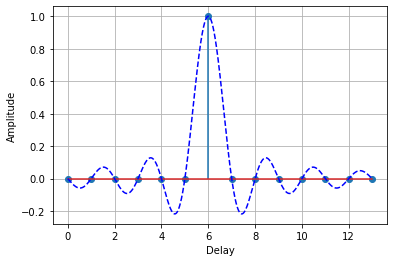
\includegraphics[width=\linewidth]{./figures/screenshots/Fractional_delay_6}
		\caption{Integer delay of 6 samples.}
	\end{subfigure}
	\hskip 5mm
	\begin{subfigure}{.4\linewidth}
		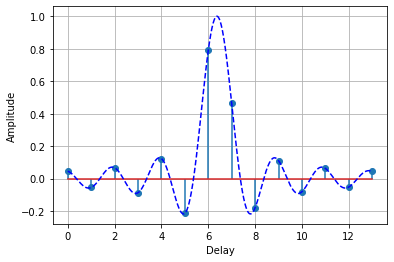
\includegraphics[width=\linewidth]{./figures/screenshots/Fractional_delay_637}
		\caption{Fractional delay of 6.37 samples.}
	\end{subfigure}
	\caption{
		FIR filters for integer and fractional delays.
		\label{fig:fractional-delay-sinc-plot}
	}
\end{figure}

As mentioned in \ref{sec:discrete-time-model} a FIR filter can be used to simulate discrete-time models of multipath fading. But with FIR filters the delays can only be integer multiples of the sample rate. When the delays are non integer an approximation needs to be done, that is because FIR filters have a transfer function of the form
\begin{equation} \label{eqn:transfer-function-fir}
	H(j\omega) = \sum_{n = 0}^{N} h(n) e^{-j\omega nT}
	\quad \text{commonly written as} \quad
	H(z) = \sum_{n = 0}^{N} h(n) z^{-n},
\end{equation}
but a non integer delay of \(\tau\) in the frequency domain is \(H_\tau(j\omega) = e^{-j\omega \tau}\). There are multiple ways to find coefficients \(h(n)\) that approximate \(H_\tau\), in this case the least squares method was used by minimizing the error function
\begin{equation}
	E(j\omega) = H(j\omega) - H_\tau(j\omega).
\end{equation}
The least square method plus the assumption of finite bandwidth and the requirement of causality gives the following rule for computing the FIR filter coefficients:
\begin{equation}
	h(n)= \begin{cases}
		\sinc (n - \tau) & 0 \leq n \leq N \\ 
		0 & \text { otherwise }
	\end{cases},
\end{equation}
where the odd order of the filter \(N\) should satisfy the condition
\begin{equation} \label{eqn:fractional-fir-length}
	N = 2 \lfloor \tau \rfloor + 1
\end{equation}
for a minimal error in the approximation. It is worth mentioning that it is also possible to build FIR filters of even length with a different condition, or that do not satisfy \eqref{eqn:fractional-fir-length}, in which cases more consideration is required. An example of a fractional delay FIR filter is shown in \figref{fig:fractional-delay-sinc-plot}.

\subsection{Statistical model} \label{sec:statistical-model}

Because as mentioned earlier it is difficult to estimate the time-dependent parameters of \(h_l(m)\) in many cases it is easier to model the components of the CIR as stochastic processes, thus greatly reducing the number of parameters \cite{Messier,Mathis}. This is especially effective for channels that are constantly changing, because by the central limit theorem the cumulative effect of many small changes tends to a normal distribution.

% \skelpar[3]{Assumptions of the model}
Before discussing the models themselves, their underlying statistical assumptions need to be considered. In the literature the so called WSSUS assumptions are made, which for a discrete time CIR \(h_l(m)\) can be formulated as
\begin{subequations}
	\begin{align}
		R_{l} (k) &= \E{h_l(m) h_l^*(m+k)}, \text{ and } \label{eqn:stat-wss} \\
		0 &= \E{h_l(m) h_k^*(m)} \text { for } l \neq k. \label{eqn:stat-us}
	\end{align}
\end{subequations}
Equation \eqref{eqn:stat-wss} states that the fading CIR is a \emph{wide sense stationary} stochastic process, while \eqref{eqn:stat-us} is the \emph{uncorrelated scattering} assumption, which says that the path do not interfere with each other. The latter is more realistic than the former, but WSS is still useful as it considerably simplifies the mathematical formulation \cite{Messier}.

\paragraph{NLOS case}

Recall that \(h(\tau, t)\) is a function of time because \(c_k\) and \(\tau_k\) change over time. The idea of the statistical model is to replace the cumulative change caused by \(c_k\) and \(\tau_k\) (which are difficult to estimate) with a single random variable \(f\). This is done as follows.

Multipath fading is a form of multiplicative noise, as mathematically confirmed by the fact that convolving a complex baseband signal \(e^{j\omega_c t}\) with the fading CIR \(h(\tau, t)\) gives
\begin{equation}
	e^{j\omega_c \tau} * h(t, \tau) = \sum_k c_k(t) e^{j\omega_c(\tau - \tau_k(t))}
	= e^{j\omega_c \tau} \sum_k c_k(t) e^{-j\omega_c \tau_k(t)}
	= e^{j\omega_c \tau} \cdot f(t).
\end{equation}
If there is no line of sight (NLOS), it is reasonable to assume that all path have more or less the same attenuation, i.e. all \(c_k\) are the same. Another reasonable assumption in this case is that all paths are equally likely to be taken, or in other words the delays \(-\omega_c \tau_k\) can be replaced with random variables \(\vartheta_k\) that are uniformly distributed on \([0,2\pi)\) \cite{Hoher2013,Mathis}. Finally, assuming that there are infinitely many paths the random variable for the multiplicative fading noise becomes
\begin{equation}
	f = \lim_{N\rightarrow\infty} \frac{1}{\sqrt{N}}
		\sum_{k=1}^{N} e^{j \vartheta_k },
\end{equation}
where the \(c_k\) where omitted, since they are assumed to be all equal. The factor \(1/\sqrt{N}\) is introduced such that \(\expectation \{|f|^2\} = 1\). It then can be shown that the probability density function of \(|f|\) is
\begin{equation}
	p(a)= 2a e^{-a^2}, \text{ or } |f| \sim \mathcal{R},
\end{equation}
i.e. the amplitude of \(f\) is \emph{Raileigh} distributed.

\begin{figure}
	\centering
	\begin{subfigure}{.45\linewidth}
		\skelfig
		\caption{NLOS, Rayleigh}
	\end{subfigure}
	\hskip 5mm
	\begin{subfigure}{.45\linewidth}
		\skelfig 
		\caption{LOS, Rice}
	\end{subfigure}
	\caption{
		Ring of scattering objects.
		\label{fig:multipath-statistical-models}
	}
\end{figure}


\paragraph{LOS case}

In the case of the Ricean distribution model the line of side exist, which means that one of the paths have a straight communication line from the transmitter to the reviser. So there are in addition to the Rayleight model direct components, whish are also gaussian distributed.

\begin{equation} \label{eqn:rician fading}
	f(t) = \sqrt{\frac{K}{K+1}}+\lim_{N\rightarrow\infty}\frac{1}{\sqrt{K+1}} \frac{1}{\sqrt{N}}\sum_{n=1}^{N} e^{j(\Theta +2\pi jf t)}.
\end{equation}  

The factor \(K\) named Ricean factor it is the ratio of the line of side power to the average power of the distributed components.
The Phase for the strait line component has no influences for the Random process therefore there set to zero. In the case when \(K = 0 \)
the Rician distribution becomes a Rayleight distribution on the other hand when \(K\rightarrow \infty \) the distribution becomes an AWGN-channel model (additive white Gaussian noise). When \(K > 0 \) is the phase not equally distributed.

For this distribution model the expectation value for the real part is \(\E{\Re{f(t)}}=\sqrt{\frac{K}{K+1}} \) and for the imaginary part \(\E{\Im{f(t)}}=0\) 

So the probability function of the amplitude in this case is:
\begin{equation} \label{eqn:rician_fading_probabilety_dencety}
	p(a)= 2a(1+K)\exp{(-K-{a}^2(K+1))}\cdot I_0(2a\sqrt{K(1+K)})
\end{equation}

Where \(I_0\) the zero ordered modified besselfunction represent.

\begin{equation}
	\Re{h_l(n)}, \Im{h_l(n)}
	\sim \mathcal{N} \left( \frac{A_l}{\sqrt{2}}, \frac{1}{2} \sigma_l^2 \right)
\end{equation}
\skelpar[4]
